\documentclass[border=10pt]{standalone}

\usepackage{tikz}
\usepackage{tikzsymbols}
\usetikzlibrary{calc,patterns,shapes.geometric}

\def\centerarc[#1](#2)(#3:#4:#5){\draw[#1] ($(#2)+({#5*cos(#3)},{#5*sin(#3)})$) arc (#3:#4:#5);}

\begin{document}
	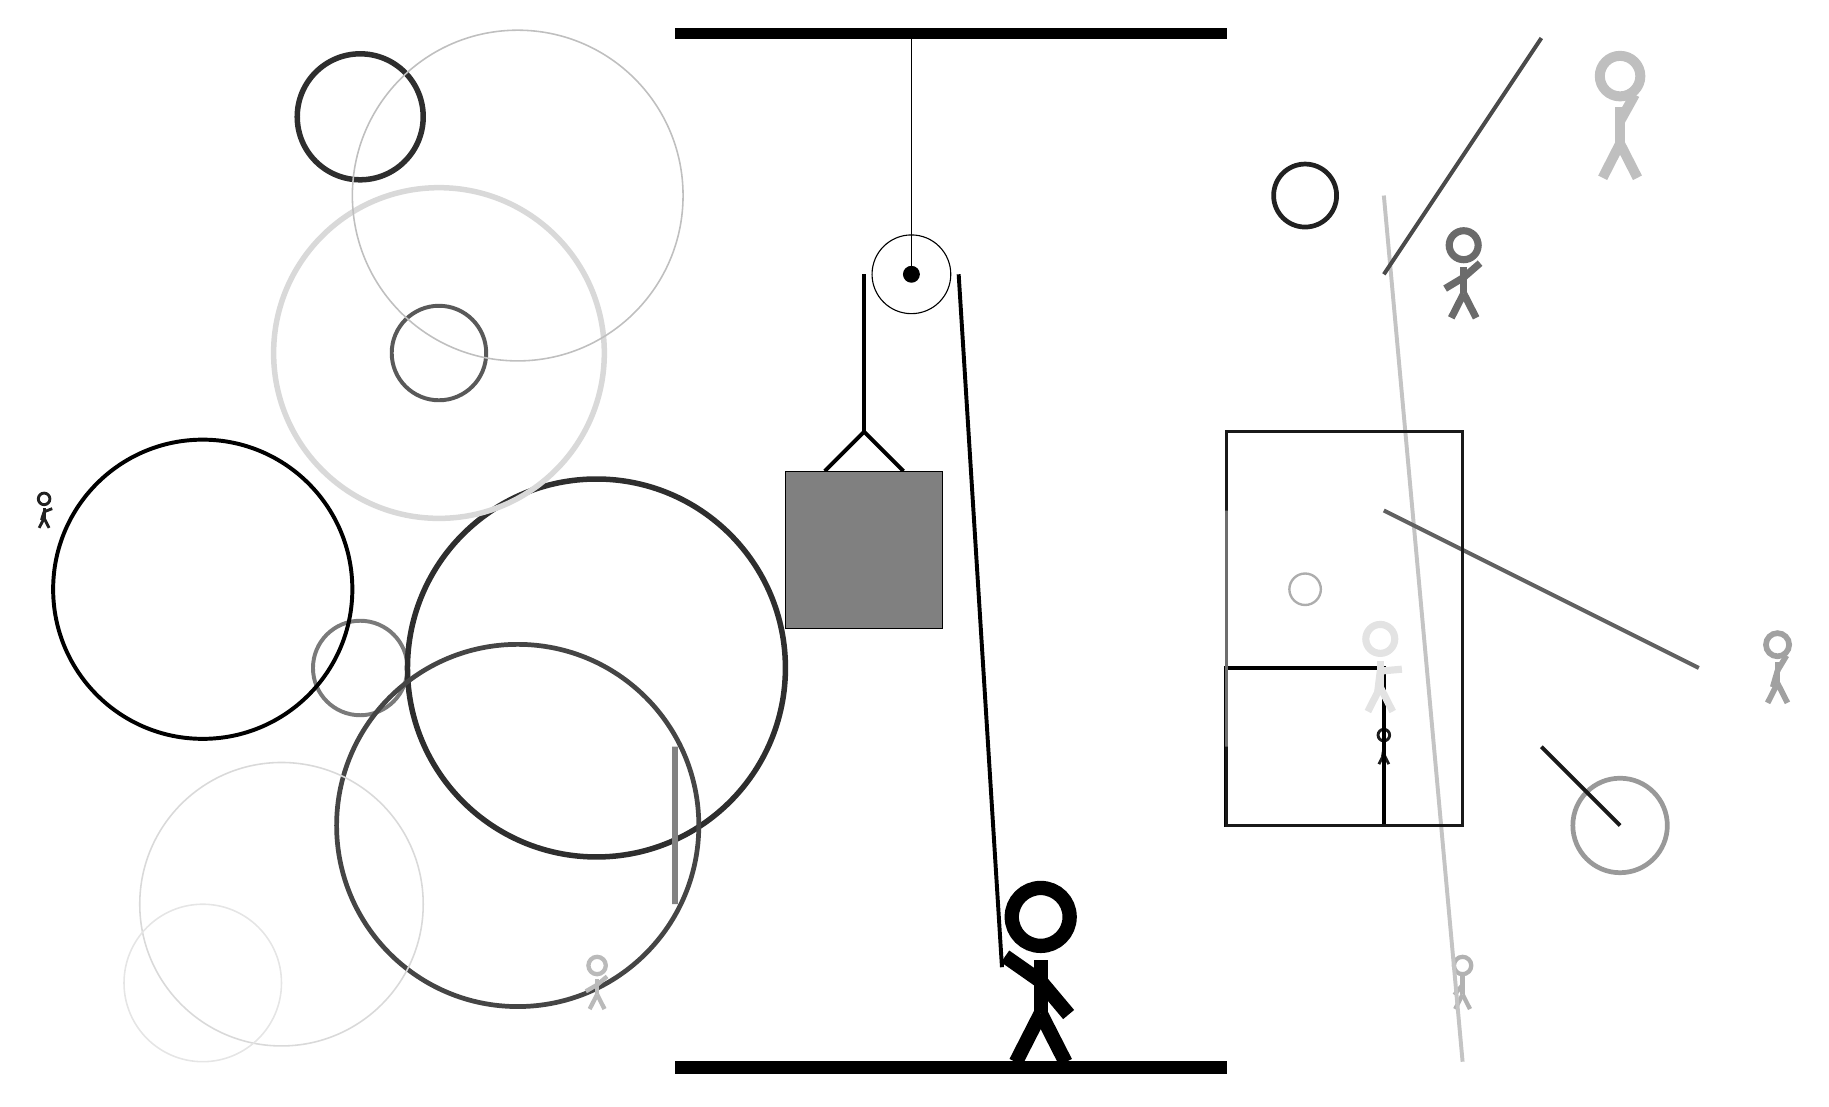
\begin{tikzpicture}
		%%%%% START %%%%%
		
		\draw[fill=black] (-2, 10) rectangle (5, 10.125);
		
		\draw (1, 7) circle (0.5);
		\draw[fill=black] (1, 7) circle (0.1);
		\draw (1, 10) -- (1, 7);
		
		\draw[line width=0.5mm] (-0.1, 4.5) -- (0.4, 5.0) -- (0.9, 4.5);
		\draw[fill=black!50] (-0.6, 4.5) rectangle (1.4, 2.5);
		
		\draw [line width=0.7mm, color=black!82](-6, 9) circle (0.8);
		
		\node[line width=0.5mm, color=black!89] at (7, 1) {\Strichmaxerl[2][81][87]};
		\draw [line width=0.5mm, color=black!52](-6, 2) circle (0.6);
		\node[line width=0.3mm, color=black!58] at (8, 7) {\Strichmaxerl[5][31][41]};
		\draw [line width=0.7mm, color=black!82](-3, 2) circle (2.4);
		
		\node[line width=0.6mm, color=black!87] at (-10, 4) {\Strichmaxerl[2][72][21]};
		
		\node[line width=0.4mm, color=black!30] at (8, -2) {\Strichmaxerl[3][51][90]};
		\node[line width=0.4mm, color=black!37] at (12, 2) {\Strichmaxerl[4][74][59]};
		\draw[line width=0.5mm, color=black!23](7, 8) -- (8, -3);
		\draw[line width=0.7mm, color=black!49] (-2, 1) rectangle (-2, -1);
		
		\draw[line width=0.5mm, color=black!100] (7, 0) rectangle (5, 2);
		\draw [line width=0.6mm, color=black!73](-4, 0) circle (2.3);
		\node[line width=0.3mm, color=black!27] at (-3, -2) {\Strichmaxerl[3][30][40]};
		\draw [line width=0.3mm, color=black!32](6, 3) circle (0.2);
		\draw[line width=0.5mm, color=black!62](7, 4) -- (11, 2);
		\draw [line width=0.5mm, color=black!65](-5, 6) circle (0.6);
		
		\draw [line width=0.2mm, color=black!15](-7, -1) circle (1.8);
		
		\draw [line width=0.6mm, color=black!40](10, 0) circle (0.6);
		\draw[line width=0.4mm, color=black!90] (5, 0) rectangle (8, 5);
		\node[line width=0.2mm, color=black!11] at (7, 2) {\Strichmaxerl[5][83][5]};
		\draw [line width=0.2mm, color=black!10](-8, -2) circle (1.0);
		
		\draw [line width=0.7mm, color=black!15](-5, 6) circle (2.1);
		
		\draw[line width=0.5mm, color=black!90](9, 1) -- (10, 0);
		\draw[line width=0.4mm, color=black!57] (5, 1) rectangle (5, 4);
		\draw [line width=0.6mm, color=black!87](6, 8) circle (0.4);
		
		\node[line width=0.3mm, color=black!25] at (10, 9) {\Strichmaxerl[7][90][61]};
		\draw [line width=0.5mm, color=black!100](-8, 3) circle (1.9);
		\draw [line width=0.2mm, color=black!25](-4, 8) circle (2.1);
		
		\draw[line width=0.5mm, color=black!71](7, 7) -- (9, 10);
		
		\draw[line width=0.5mm] (0.4, 7) -- (0.4, 5.0);
		\centerarc[line width=0.5mm](1, 7)(0:180:0.6);
		\draw[line width=0.5mm](1.6, 7) -- (2.15, -1.8);
		
		\node at (2.6, -1.9) {\Strichmaxerl[10][-35][-50]};
		
		\draw[fill=black] (-2, -3) rectangle (5, -3.15);
		
		%%%%% END %%%%%
	\end{tikzpicture}
\end{document}